
\chapter{Leveraging layout for sparse attention}
\label{chapter:skim-attention}

\renewcommand{\leftmark}{\spacedlowsmallcaps{Leveraging layout for sparse attention}}

\begin{chapabstract}
	{\em    
        While multimodal pre-training techniques prove effective, their development is not primarily driven by efficiency considerations. Built upon the Transformer architecture, these models suffer from the quadratic complexity of self-attention, hindering their applicability to long documents. In this work, our focus lies in exploiting layout in a computationally efficient manner. In particular, we explore two research questions: 
        \begin{enumerate}
            \item Is it possible to determine attention from layout only? 
            \item Can layout help reduce the complexity of self-attention? 
        \end{enumerate}
        Motivated by human reading strategies, we present Skim-Attention, a new attention mechanism that takes advantage of the structure of the document and its layout. Skim-Attention only attends to the 2-dimensional position of the words in a document. To exploit this mechanism, we introduce Skimformer and Skimming Mask, two frameworks for integrating Skim-Attention into the Transformer architecture. Our experiments show that Skim-Attention obtains a lower perplexity than prior works, while being more computationally efficient. We also show how Skim-Attention can be used off-the-shelf as a mask for any \ac{PLM}, allowing to improve their performance while restricting attention. Finally, we show the emergence of a document structure representation in Skim-Attention.     
	\vspace*{5mm}
	
	The work in this chapter has led to the publication of a conference paper:}
	\begin{itemize}
		\item \small \fullcite{nguyen-etal-2021-skim-attention}.
	\end{itemize}
\end{chapabstract}

\ifthenelse{\boolean{skipCh6}}{\endinput}{}


\newpage

\minitoc
\chapterwithfigures{\nameref*{chapter:skim-attention}}
\chapterwithtables{\nameref*{chapter:skim-attention}}

% Despite their effectiveness, multimodal pre-training techniques are not motivated by an efficiency perspective. Layout and visual signals are mostly viewed as additional features that boost performance, and each token is still contextualized with respect to the entire input sequence. However, prior works in cognitive sciences have shown that humans use the layout as a strategy to retrieve information faster, while expending less effort \citep{britton1982effects, olive2017processing}. In this chapter, draw insights from these discoveries and exploit layout in a manner akin to humans, as this can be key to a successful model coping with long and complex documents. We raise two research questions: (RQ1) Is it possible to learn attention using layout only? (RQ2) Can layout help reduce the complexity of self-attention? 

As seen in Chapter~\ref{chapter:related-document-understanding}, Transformer-based joint pre-training of text, layout and images has allowed models to reach state-of-the-art performance in a number of document understanding tasks. However, multimodal pre-trained models suffer from very high computational and memory costs due to the quadratic complexity inherent to Transformers, rendering them unable to process long documents. In most approaches, layout is considered an additional feature (\textit{e.g.}, integrating 2D coordinates as an extension of 1D positions) that enhances performance, and each token is still contextualized with respect to the entire input sequence. Yet, layout stands as a distinct modality alongside language. The conventional approach of treating layout as a special positional feature leads to a lack of cross-modal interaction between layout and text. This limitation has the potential to impede the model's understanding of the role that layout plays in semantic expression.

% Understanding how the author is presenting and organizing information frees up memory and processing resources allowing the reader more capacity to comprehend content
% According to Meyer (1987), text structure instruction might beeffective for improving reading comprehension
It has been shown that a well-designed layout results in less cognitive effort \citep{kieras1978beyond, britton1982effects, olive2017processing} and facilitates comprehension of the conveyed information by helping identify the document type and its constituents, as well as providing cues regarding relationships between elements \citep{meyer1980use, wright1999psychology}. Semiotic research assumes that readers scan the document before taking a closer look at certain units \citep{kress1996reading}, a claim supported by eye-tracking experiments on newspapers \citep{leckner2012presentation}. Inspired by these research findings, we claim that one does not need to have read each word in a document page to be able to understand a specific paragraph. Therefore, we argue that, to efficiently process long documents, it is a waste of effort and computation to contextualize a token with respect to the entire input sequence. To shift towards processing long documents with awareness of their structure, we propose to leverage layout in a more intuitive and efficient way, resembling human cognition. We argue that this approach can be key to a model coping with long and complex documents.

We delve into two research questions:

\begin{enumerate}
    \item Can attention be effectively learned using layout information exclusively?
    \item Can layout be used to reduce the complexity of self-attention?
\end{enumerate}

In addressing these questions, we propose Skim-Attention, a new self-attention mechanism that relies solely on the 2D position of tokens in the page, independently of their semantics. To exploit this mechanism, we introduce Skimformer and Skimming Mask, two frameworks for integrating Skim-Attention into Transformer models. Skimformer is an end-to-end Transformer language model that computes the Skim-Attention scores just once and uses them across each layer of a text-based Transformer encoder. This designs mirrors human reading strategies, where the model skims through the document to extract its structure, and reads the contents based on the prior structural understanding. Moreover, Skimformer can be adapted for long-range Transformers to model longer documents. On the other hand, Skimming Mask uses Skim-Attention as a masking mechanism to sparsify attention within any Transformer language model. Each token's attention is restricted to at most $k$ tokens, as identified by Skim-Attention. This approach allows for a smaller context length, thereby leading to more efficient computation.

In this chapter, we first present a simple cognitive experiment that highlights the fundamental role of layout in humans' comprehension of documents. Then, we introduce the Skim-Attention mechanism and its integration into Transformer language models. Finally, we showcase the quantitative and qualitative benefits of our approach.


\section{Preliminary Experiments: Human Evaluation}
\label{section:human-evaluation}

How much does the document layout help in comprehending long textual contents? How faster is it for humans to find information in documents when layout is provided? To answer these questions, we conduct a simple cognitive experiment wherein we measure the amount of time needed for human annotators to extract information from both formatted and plain-text documents. We hand-pick four document pages from the DocBank dataset \citep{li2020docbank}, and create a plain-text version out of each of these documents by serializing them. We create two basic questions for each document, and ask four annotators to answer them. Half of the time, annotators are given access to the full layout, while the other half, they are limited to plain text only (i.e., no layout nor formatting).

\begin{figure}[!htbp]
    \centering
      \begin{subfigure}[b]{0.24\textwidth}
        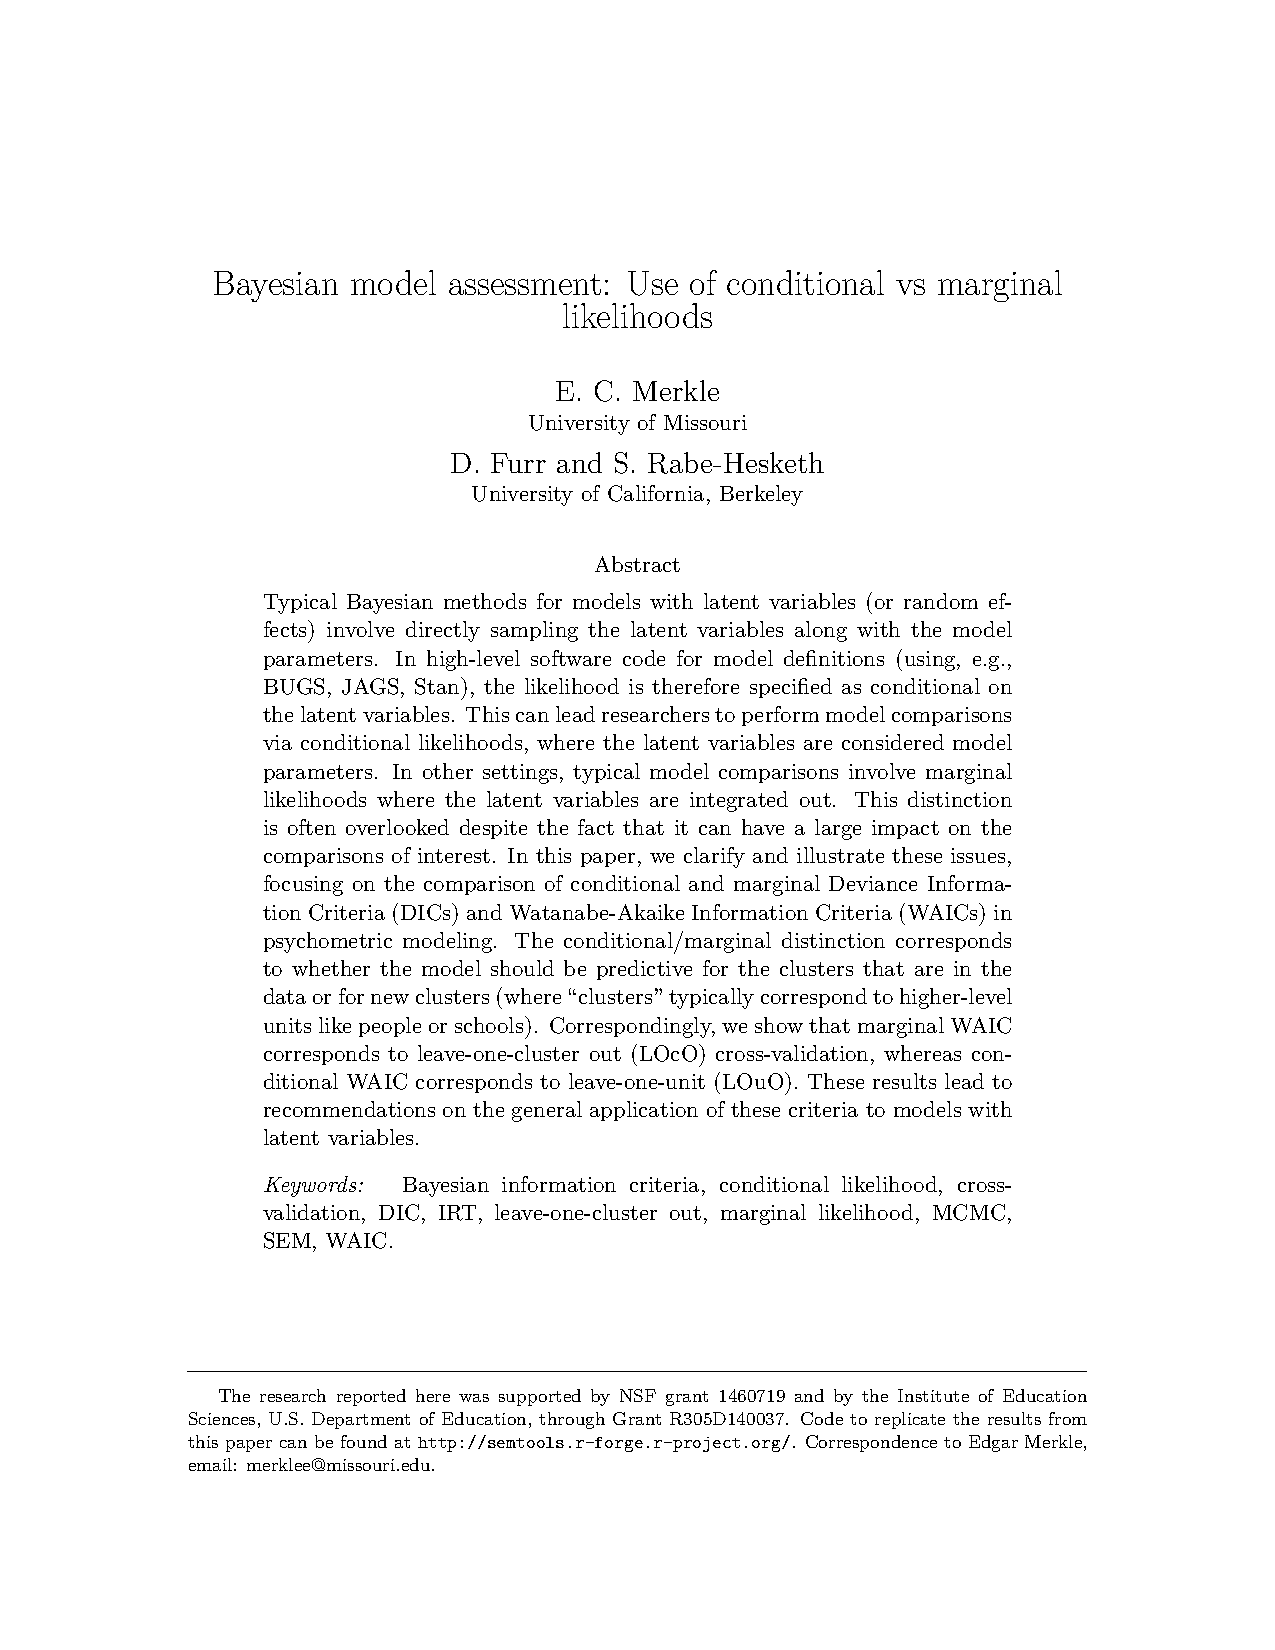
\includegraphics[width=\textwidth]{images/chapter3/formatted_sample1.pdf}
        % \caption{}
      \end{subfigure}
      \hfill
    %   \hspace{0.25em}
      \begin{subfigure}[b]{0.24\textwidth}
        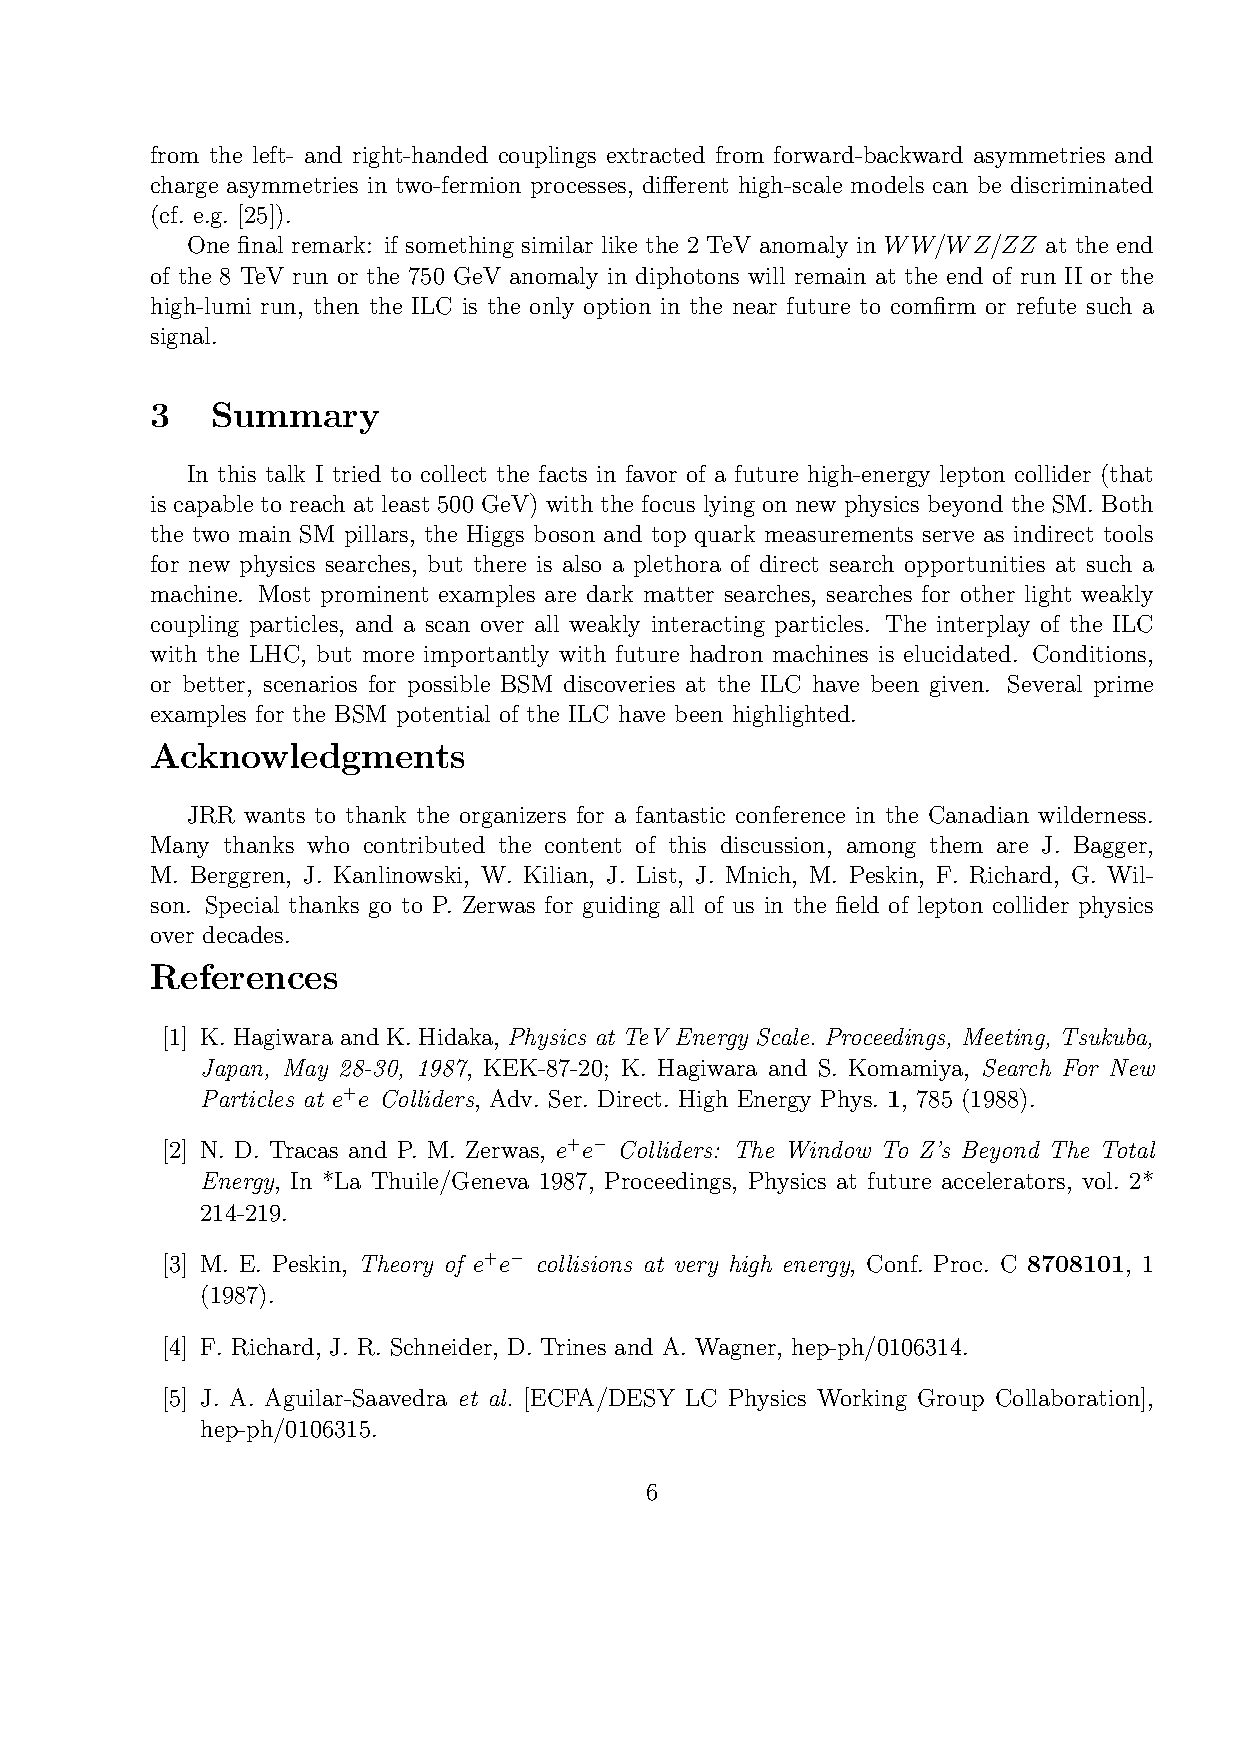
\includegraphics[width=\textwidth]{images/chapter3/formatted_sample2.pdf}
        % \caption{}
      \end{subfigure}
      \begin{subfigure}[b]{0.24\textwidth}
        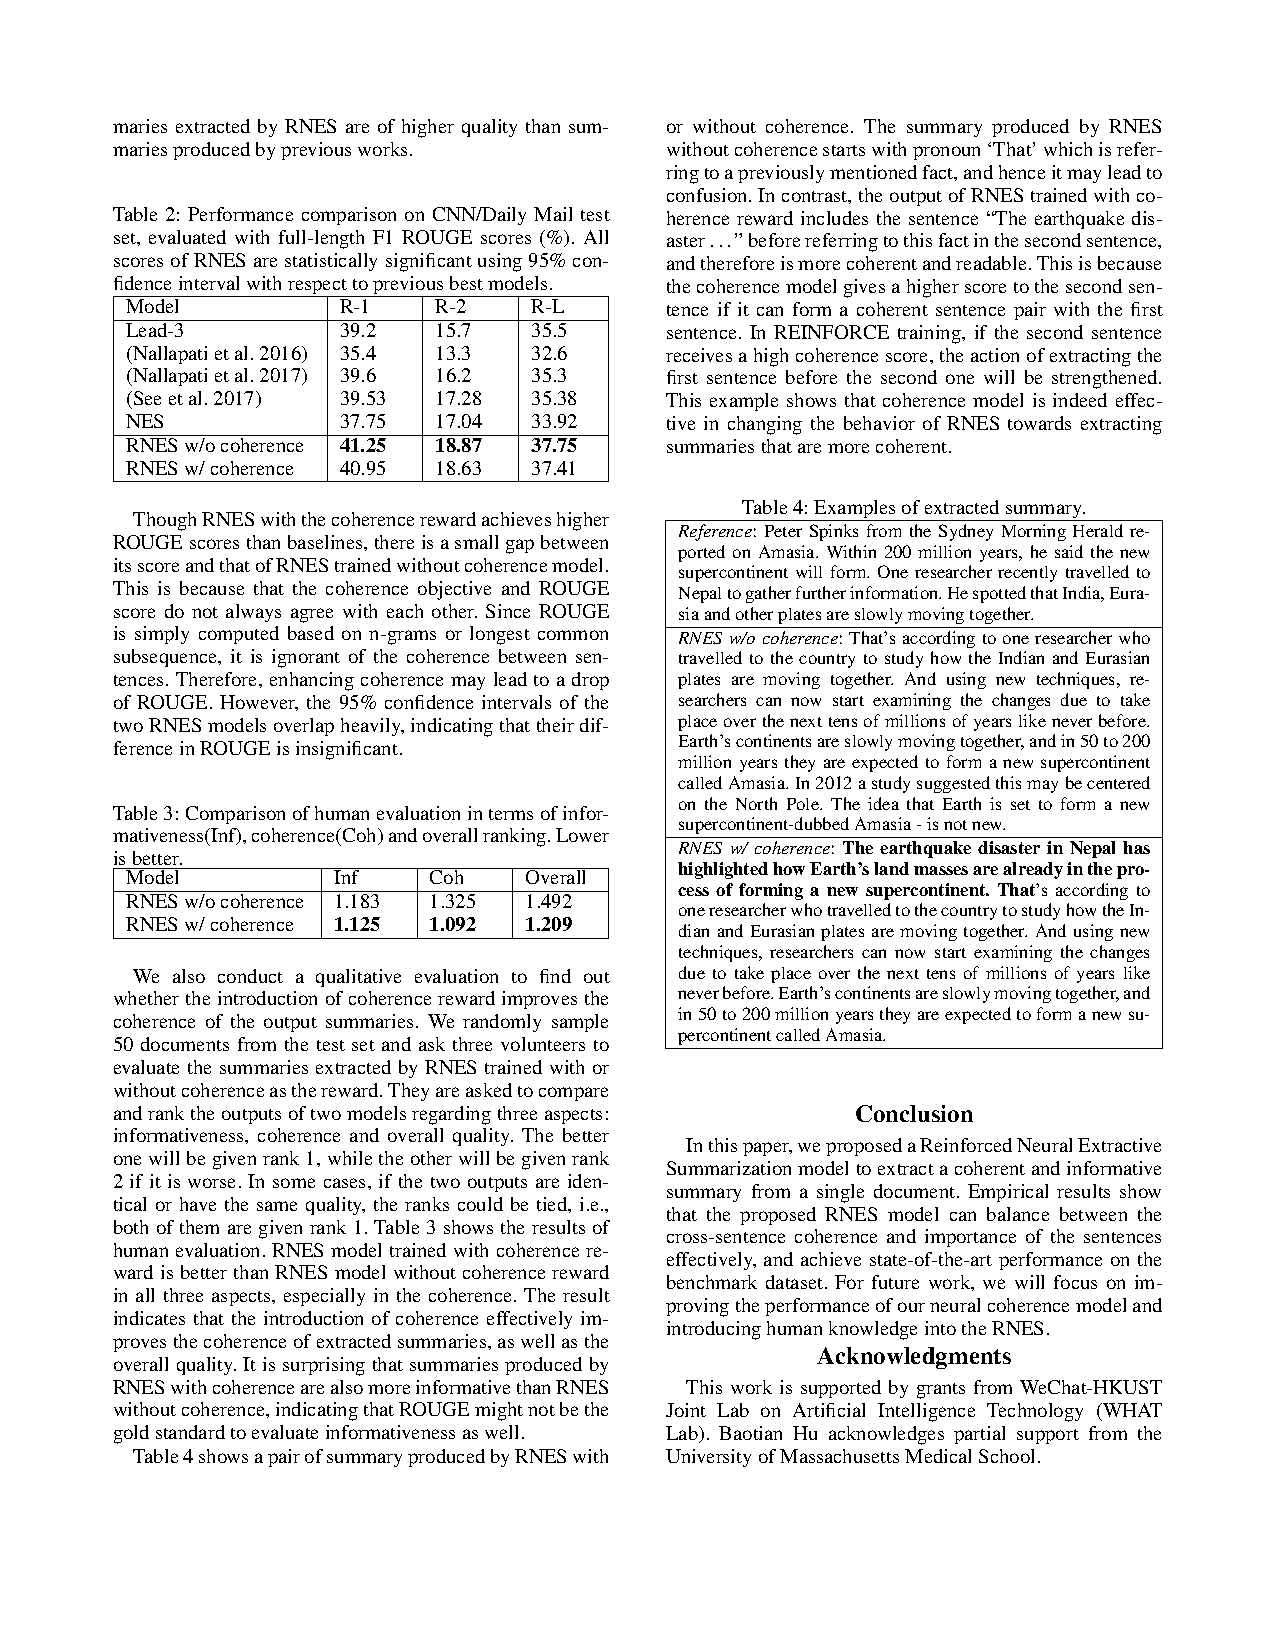
\includegraphics[width=\textwidth]{images/chapter3/formatted_sample3.pdf}
        % \caption{}
      \end{subfigure}
      \begin{subfigure}[b]{0.24\textwidth}
        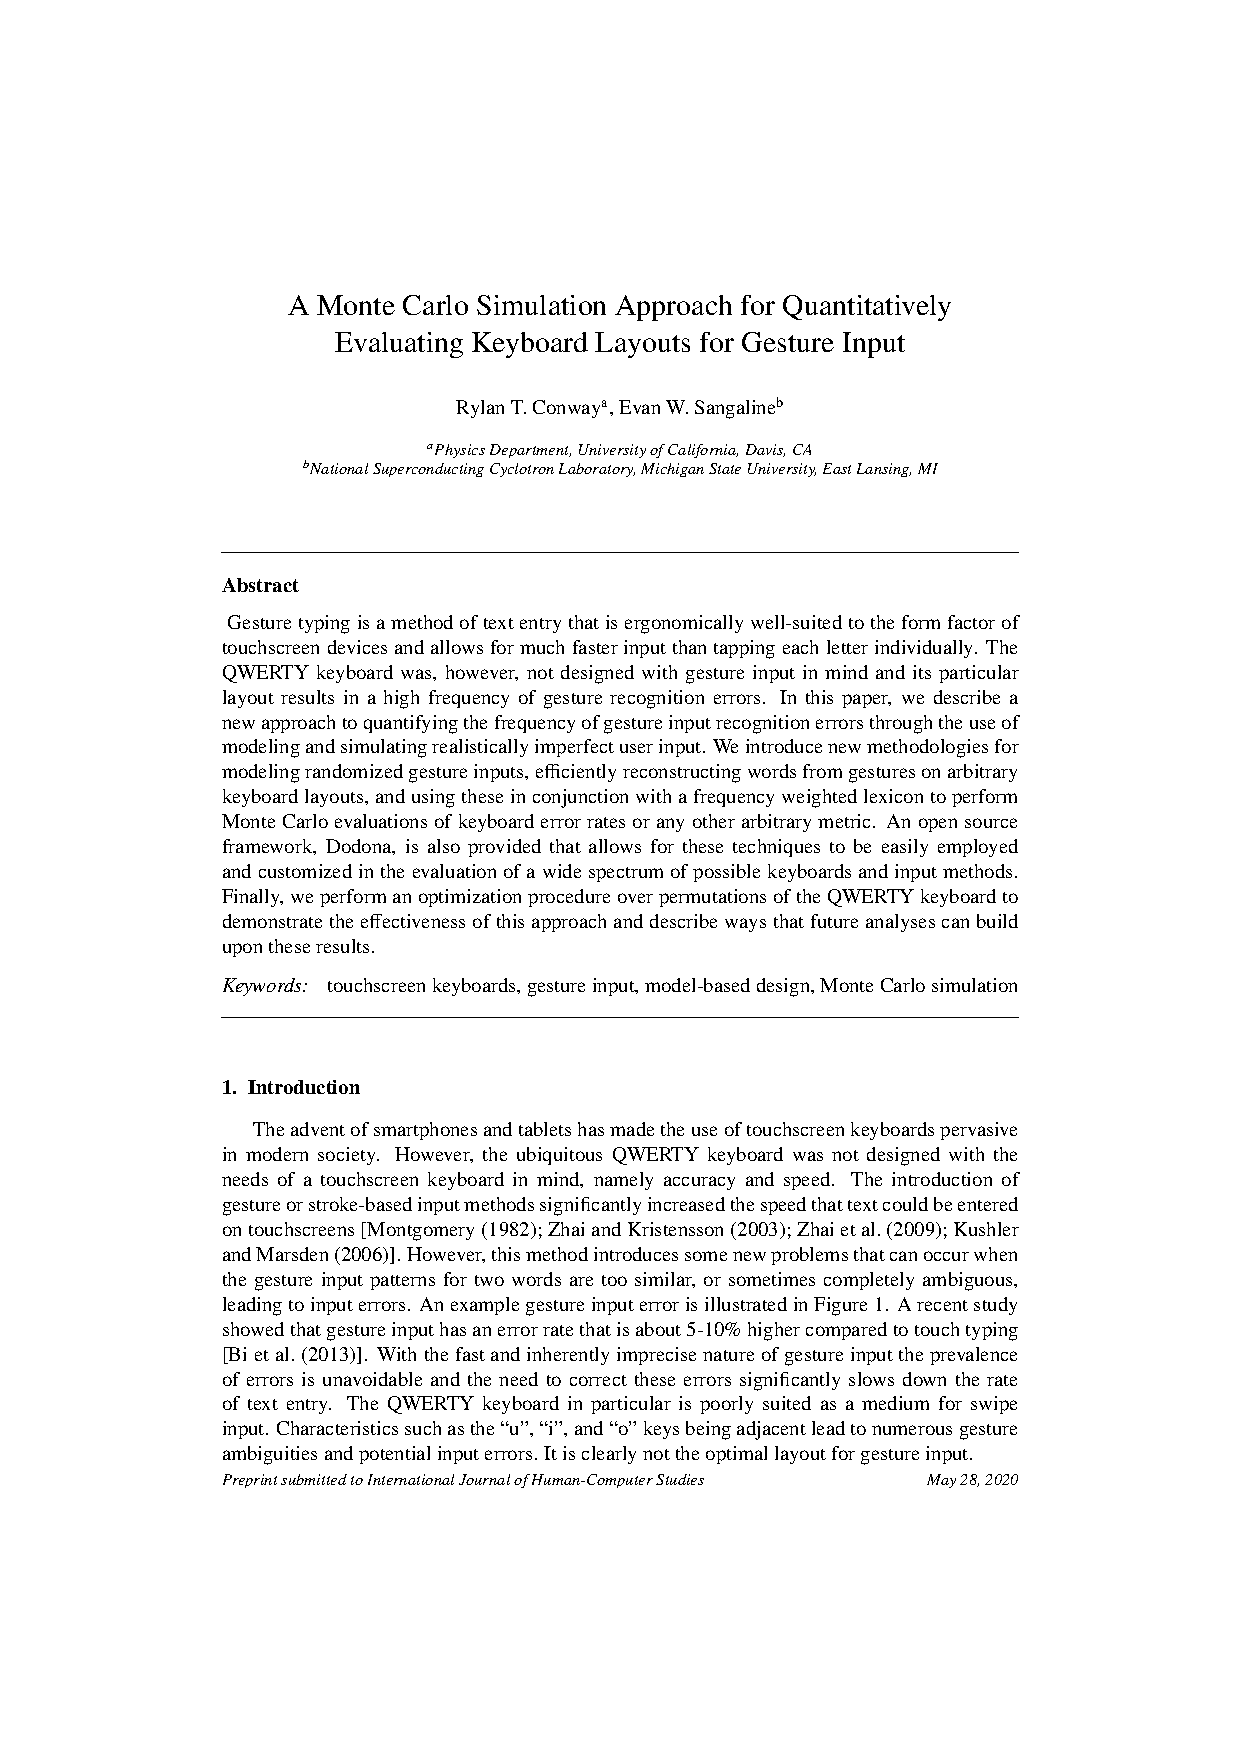
\includegraphics[width=\textwidth]{images/chapter3/formatted_sample4.pdf}
        % \caption{}
      \end{subfigure}
      \caption{Documents selected for our preliminary cognitive experiment.}
      \label{fig:samples-chapter3}
\end{figure}

Table~\ref{tab:human-eval} reports the average time needed to retrieve information from the documents. We find that it is 2.5 times faster to answer questions from the formatted documents, and that the variability in the results is much lower in this case. These results support the hypothesis that \emph{less cognitive effort} is spent when the document is formatted, emphasizing the importance of layout information in reading comprehension.

We believe that machines could benefit from the the document layout, just like humans, as a strategy to retrieve information faster while expending less effort. In particular, layout information could be of great help in reducing the cost of self-attention in Transformer models (Section~\ref{subsubsection:training-speed-memory-usage}) and facilitating the emergence of a document structure representation (Section~\ref{subsection:attention-visualization}).

\begin{table}
\centering \small
    \begin{tabular}{crr}
        \hline
                   & \textbf{Average} & \textbf{Standard Deviation} \\
        \hline 
        Formatted  & 6.05  & 1.73 \\
        Plain-text & 15.18 & 9.06 \\
        \hline
    \end{tabular}
\caption{Average (std) time (in seconds) required to answer questions from documents, depending on whether layout is provided.}
\label{tab:human-eval}
\end{table}

\section{Skim-Attention: A Novel Layout-Aware Attention Mechanism}

In light of the aforementioned cognitive experiment, it is clear that layout is of utmost importance for humans to understand long documents. We propose to take layout into consideration by introducing \emph{Skim-Attention}, a self-attention module that computes attention solely based on the spatial positions of tokens. To process long and layout-rich documents, we present different ways of integrating this mechanism into Transformer architectures.

\subsection{Skim-Attention Overview}

Our novel attention mechanism, Skim-Attention, views documents as collections of word bounding boxes distributed over a two-dimensional space, \textit{i.e.}, the page. In the following, we provide details on how to encode spatial positions into layout embeddings, followed by a detailed description of our attention module.

\subsubsection{Layout Embeddings}

Layout embeddings carry information about the spatial position of the tokens. Following LayoutLM \citep{xu2020layoutlm}, the spatial position of a token is represented by its bounding box in the document page image, $(x_0, y_0, x_1, y_1)$, where $(x_0, y_0)$ and $(x_1, y_1)$ respectively denote the coordinates of the top-left and bottom-right corners. We discretize and normalize them to integers in $\{0, ..., 1000\}$. Four embedding tables are used to encode spatial positions: two for the coordinate axes ($x$ and $y$), and the other two for the bounding box size (width and height). The final layout embedding of a token, $\bell \in \mathbb{R}^{d_{\ell}}$, located at position $(x_0, y_0, x_1, y_1)$ is defined by:
\vspace{-0.5cm}

\begin{equation}
\begin{split}
    \bell & = \text{LayoutEmb}_x(x_0) + \text{LayoutEmb}_y(y_0) \\
    & + \text{LayoutEmb}_x(x_1) + \text{LayoutEmb}_y(y_1) \\
    & + \text{LayoutEmb}_w(x_1 - x_0) \\
    & + \text{LayoutEmb}_h(y_1 - y_0) \\
\end{split}
\end{equation}

\subsubsection{Skim-Attention Mechanism}

% We propose Skim-Attention, an attention mechanism that leverages document layout in a novel way. 
A standard self-attention mechanism works by comparing every token in the sequence to every other token in the sequence, and reweighing the embeddings of each token to include contextual relevance (Section~\ref{subsubsection:related-pretrained-language-models-sa}). Skim-Attention diverges from standard self-attention as it operates independently from text semantics (\textit{i.e.}, token representations). Instead, Skim-Attention computes attention using \emph{only} the spatial positions of tokens, \textit{i.e.}, their layout embeddings $\bell$.

Formally, let $\bm{X}^{\ell} =  \{\bell_0, \bell_1, \ldots, \bell_n\}$ be an input sequence of layout embeddings, and $\bm{Q}^{\ell} = \bm{W}^{\ell}_q \bm{X}^{\ell}, \bm{K}^{\ell} =  \bm{W}^{\ell}_k \bm{X}^{\ell}$. The queries $\bm{Q}^{\ell}$ and keys $\bm{K}^{\ell}$ are obtained by linear transformations of the layout embeddings, following the standard attention mechanism. As in Equation~\ref{equation:related-pretrained-language-models-sa-alignment}, Skim-Attention is defined as a scaled-dot product between queries and keys, passed through a softmax operator:

\begin{equation}
\label{eq:skim-attention-matrix}
    \bm{A}^{\ell} = \text{Softmax}\left(\dfrac{\bm{Q}^{\ell}\left(\bm{K}^{\ell}\right)^\top}{\sqrt{d^{\ell}}}\right)
\end{equation}

\noindent Similar to multi-head self-attention in Transformers, Skim-Attention is decomposed in multiple heads.

Intuitively, $\bm{A}^{\ell}$ captures the correlation between two tokens based on their spatial positions: the more similar two tokens are in terms of layout embeddings, the more they should attend to each other. 

Because attention is calculated only once, using non-contextualized layout embeddings may limit Skim-Attention's ability to capture complex relationships within the document structure. Therefore, to enhance the quality of layout representations, we contextualize them by adding a small Transformer prior to computing Skim-Attention. The contextualization process allows for a more refined understanding of the relationships and dependencies within the layout.

The integration of Skim-Attention with any long-range Transformer is entirely feasible, as these approaches operate independently. We tailor our methodology by performing the long-range attention calculation once, using layout information instead of text semantics.

\subsection{Skim-Attention in Transformers}

We present two approaches to exploit Skim-Attention:
\emph{i)} \textit{Skimformer}, wherein self-attention is replaced by Skim-Attention; and \emph{ii)} \textit{Skimming Mask}, where an attention mask is built from Skim-Attention and fed to a Transformer language model.

\subsubsection{Skimformer}

\begin{figure}[h]
    \centering
    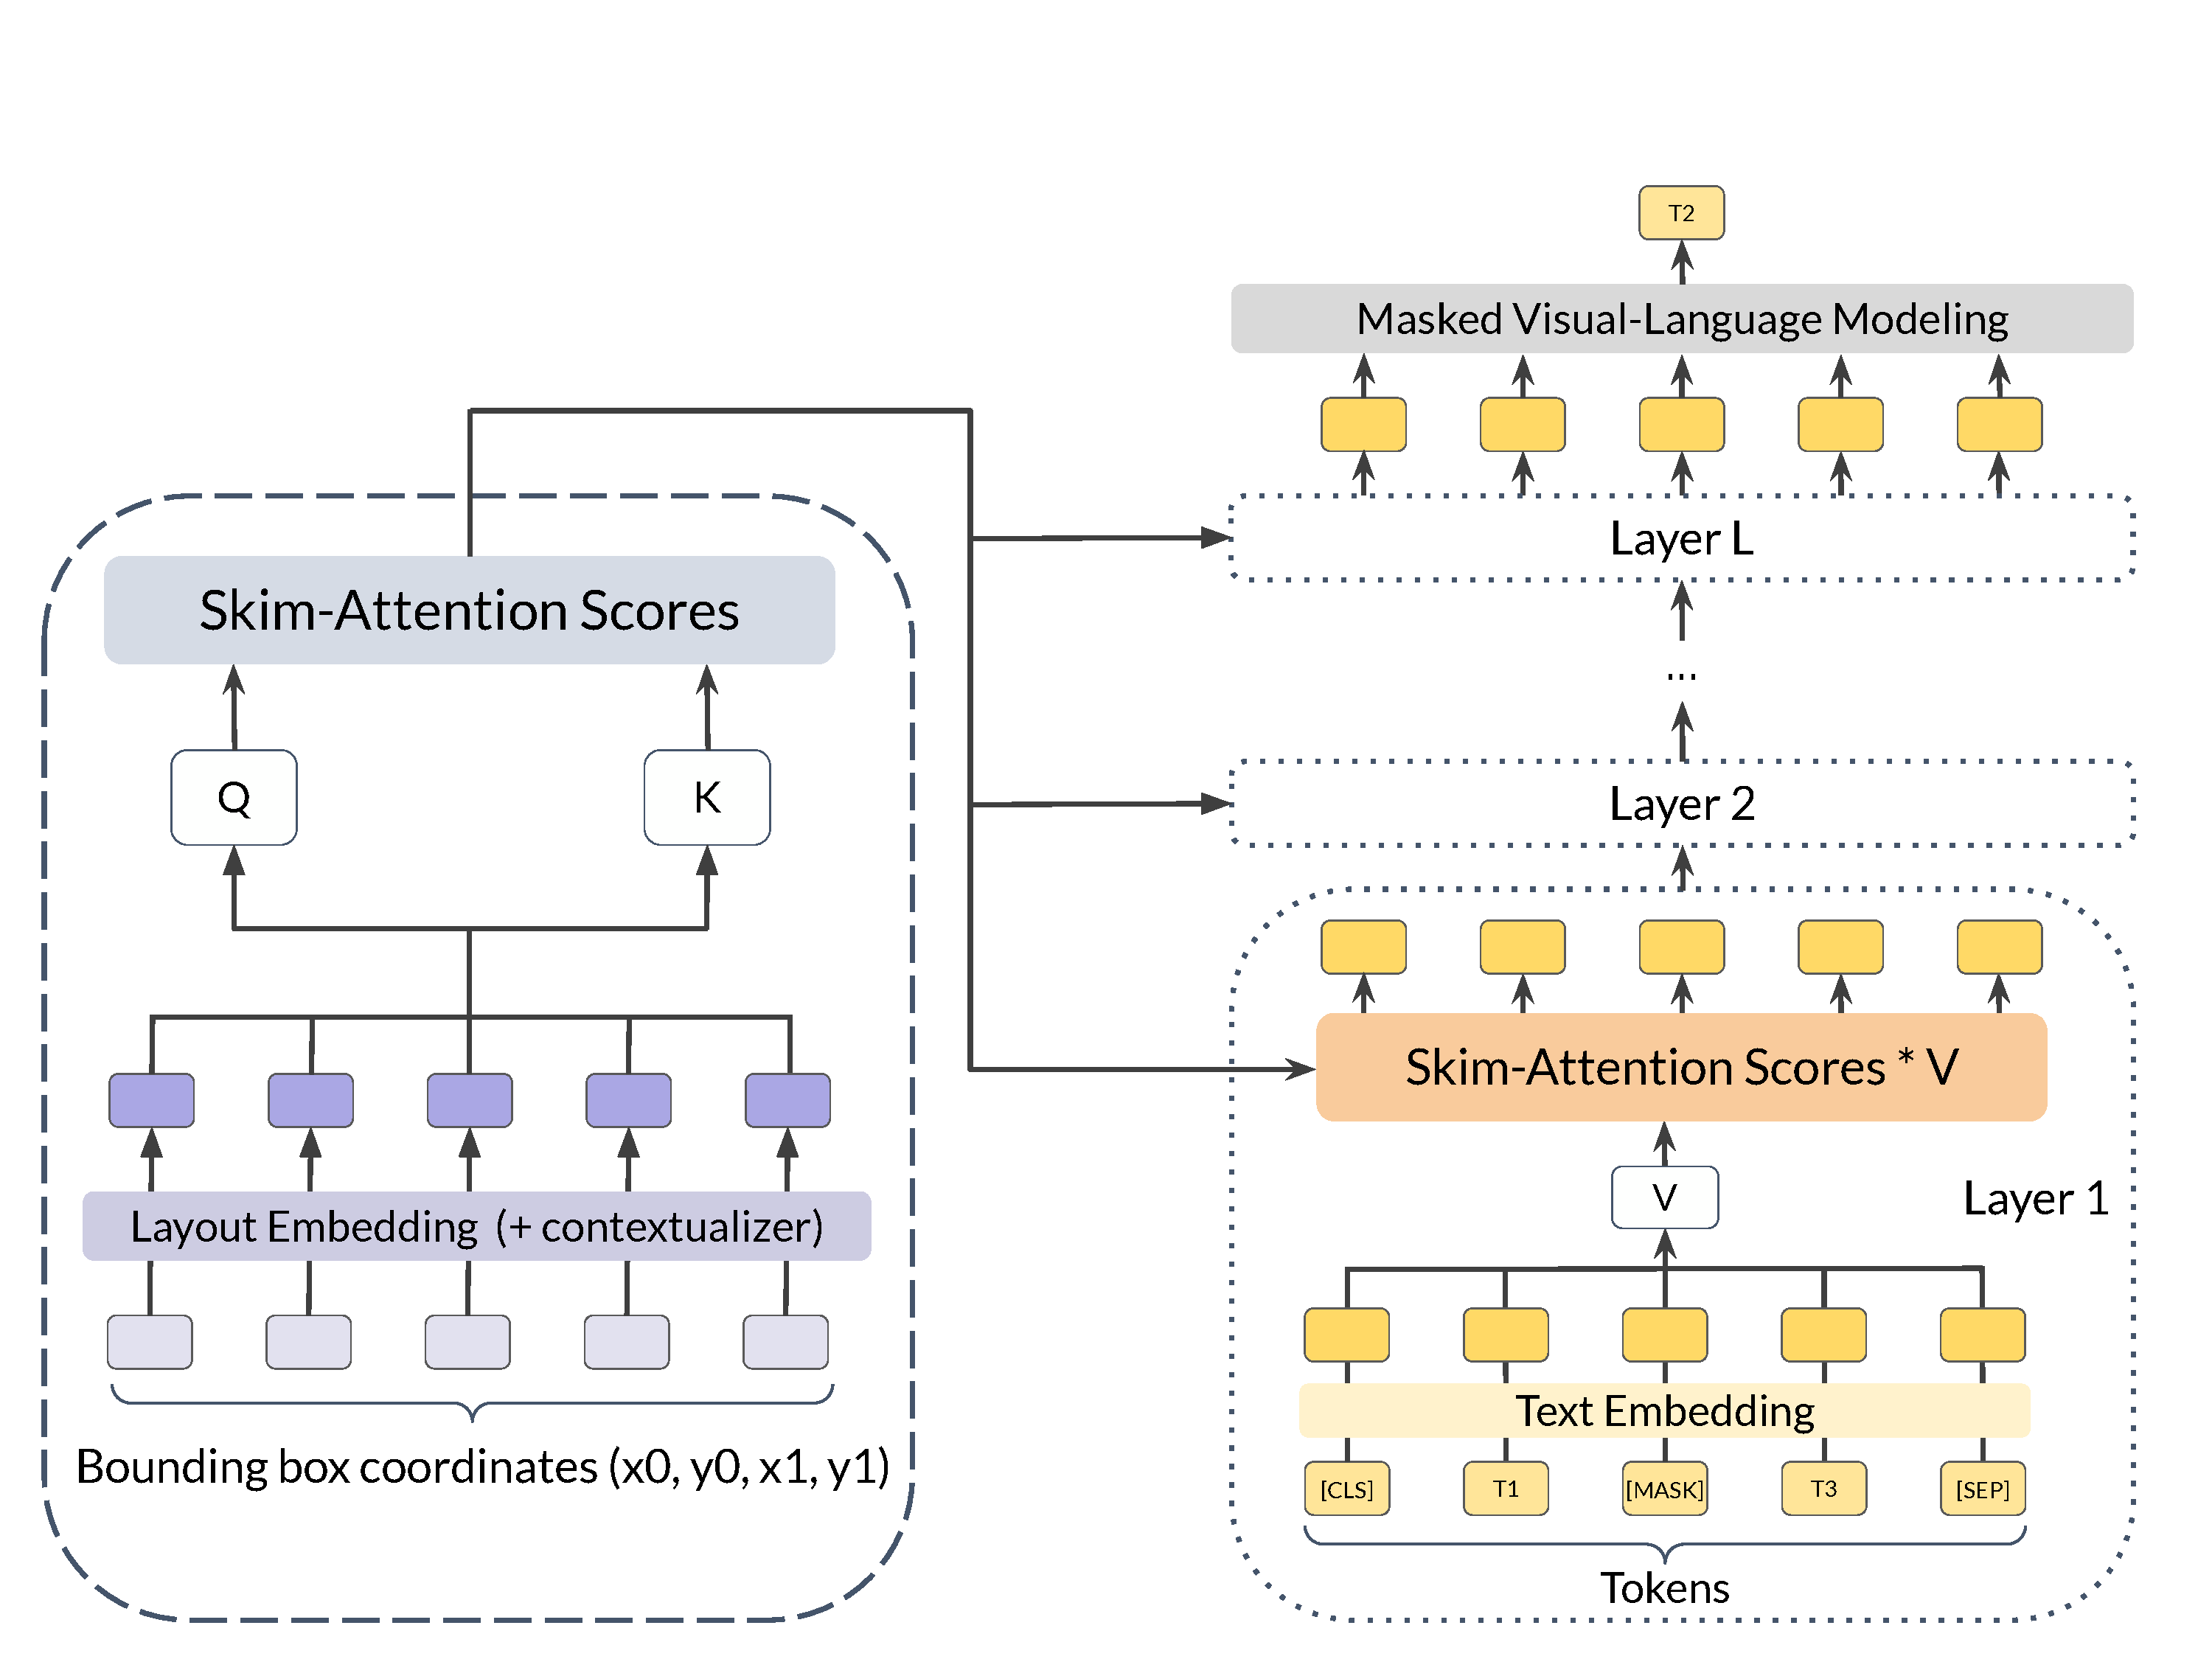
\includegraphics[width=0.7\textwidth]{images/chapter3/skimformer-architecture.pdf}
    \caption{Skimformer model architecture. The input consists of two components: a sequence of tokens (right-hand side) and a sequence of token bounding box coordinates (left-hand side). Both of these sequences are transformed into corresponding embedding sequences. Only the layout embeddings are used to compute Skim-Attention. $L$ denotes the number of Transformer encoder layers. $\bm{Q}$ and $\bm{K}$ are the queries and keys obtained by projecting the layout embeddings. $\bm{V}$ represents the values produced by projecting the encoder layers' textual inputs. The attention is solely based on token spatial positions and computed only once. The attention scores are then distributed to each layer of a Transformer encoder.}
    \label{fig:skimformer-architecture}
\end{figure}

\emph{Skimformer} is designed to answer the first research question: \textit{Is it possible to determine attention from layout only ?} Skimformer is a two-stage Transformer that replaces multiple standard self-attention layers with a single layer of Skim-Attention. Drawing inspiration from insights in cognitive science, the intuition behind this approach is to mimic how humans process a document by \emph{i)} skimming through the document to extract its structure, and \emph{ii)}  reading the contents based on the prior structural understanding. 

Skimformer is fed with a sequence of token embeddings and the corresponding sequence of layout embeddings. Because layout information implicitly reflect the reading order of documents, we do not encode the sequential positions of tokens. The model adopts a two-step approach: first, it computes the skim-attention scores once and only once using layout information alone; then it uses these attention scores across all layers of a Transformer encoder. The architecture of Skimformer is depicted in Figure~\ref{fig:skimformer-architecture}.

For a given encoder layer and a single head, the output representations $\bm{Z}$ of the standard self-attention operation becomes:

\begin{equation}
\label{eq:skim-attention-full}
	\bm{Z} = \bm{A}^{\ell} \bm{V}^{t}
\end{equation}

\noindent where $\bm{A}^{\ell}$ is the skim-attention matrix obtained through Eq.~\ref{eq:skim-attention-matrix}, and $\bm{V}^{t} = \bm{W}_{v} \bm{X}^t$ is the value matrix obtained by projecting the layer input.

More intuitively, computing skim-attention scores (Eq.~\ref{eq:skim-attention-matrix}) can be interpreted as \textit{skimming through} the document to grasp its structural aspects. Information about the semantics (contained in $\bm{V}$) is then routed based on these similarity scores. This is done via Eq.~\ref{eq:skim-attention-full} and can be seen as \textit{reading} the contents of the document, focusing on the most relevant parts guided by the skim-attention scores.

Similarly to LayoutLM, we pre-train Skimformer using \ac{MVLM}. This involves randomly masking some of the input tokens, while retaining their corresponding layout embeddings. The model is then trained to recover the masked tokens given the contexts. 

While we experimented with a standard Transformer encoder-only model, it is worth noting that any language model can be used as the backbone of Skimformer.

Albeit remaining quadratic, the time and memory cost of Skim-Attention is much lower than vanilla self-attention. Let $n$ be the maximum sequence length, $L$ the number of encoder layers, $L'$ the number of layers needed to contextualize layout representations, $d$ the dimension of the text embeddings, and $d'$ the dimension of the layout embeddings. The computational complexity is reduced from $\mathcal{O}(2Ldn^2)$ to $\mathcal{O}(L'd'n^2 + Ldn^2)$, the first term being the time required to calculate the skim-attention scores, and the second term referring to the time needed to compute the residual value for each token in the input. The memory complexity for vanilla self-attention is $\mathcal{O}(Ldn + Ln^2)$, where the first term is the memory required to store keys, queries and values, while the second represents the attention scores produced. These requirements are reduced to $\mathcal{O}((d’n + n^2) + Ldn)$, with the first term corresponding to the keys and queries, the second term representing the attention scores, and the last one corresponding to the values.

In conclusion, Skimformer is a two-stage Transformer architecture designed to determine attention from layout information alone, emulating human reading strategies by efficiently processing document structure. While enhancing efficiency, Skimformer has sub-optimal aspects. One limitation lies in the fixed nature of Skim-Attention scores across all layers, which may oversimplify the model's comprehension, potentially missing complex relationships within the document. Furthermore, a token's attention is determined solely by layout information, potentially overlooking important semantic clues that are essential to understand complex relationships.

\subsubsection{Skimming Mask}

\begin{figure}
    \centering
    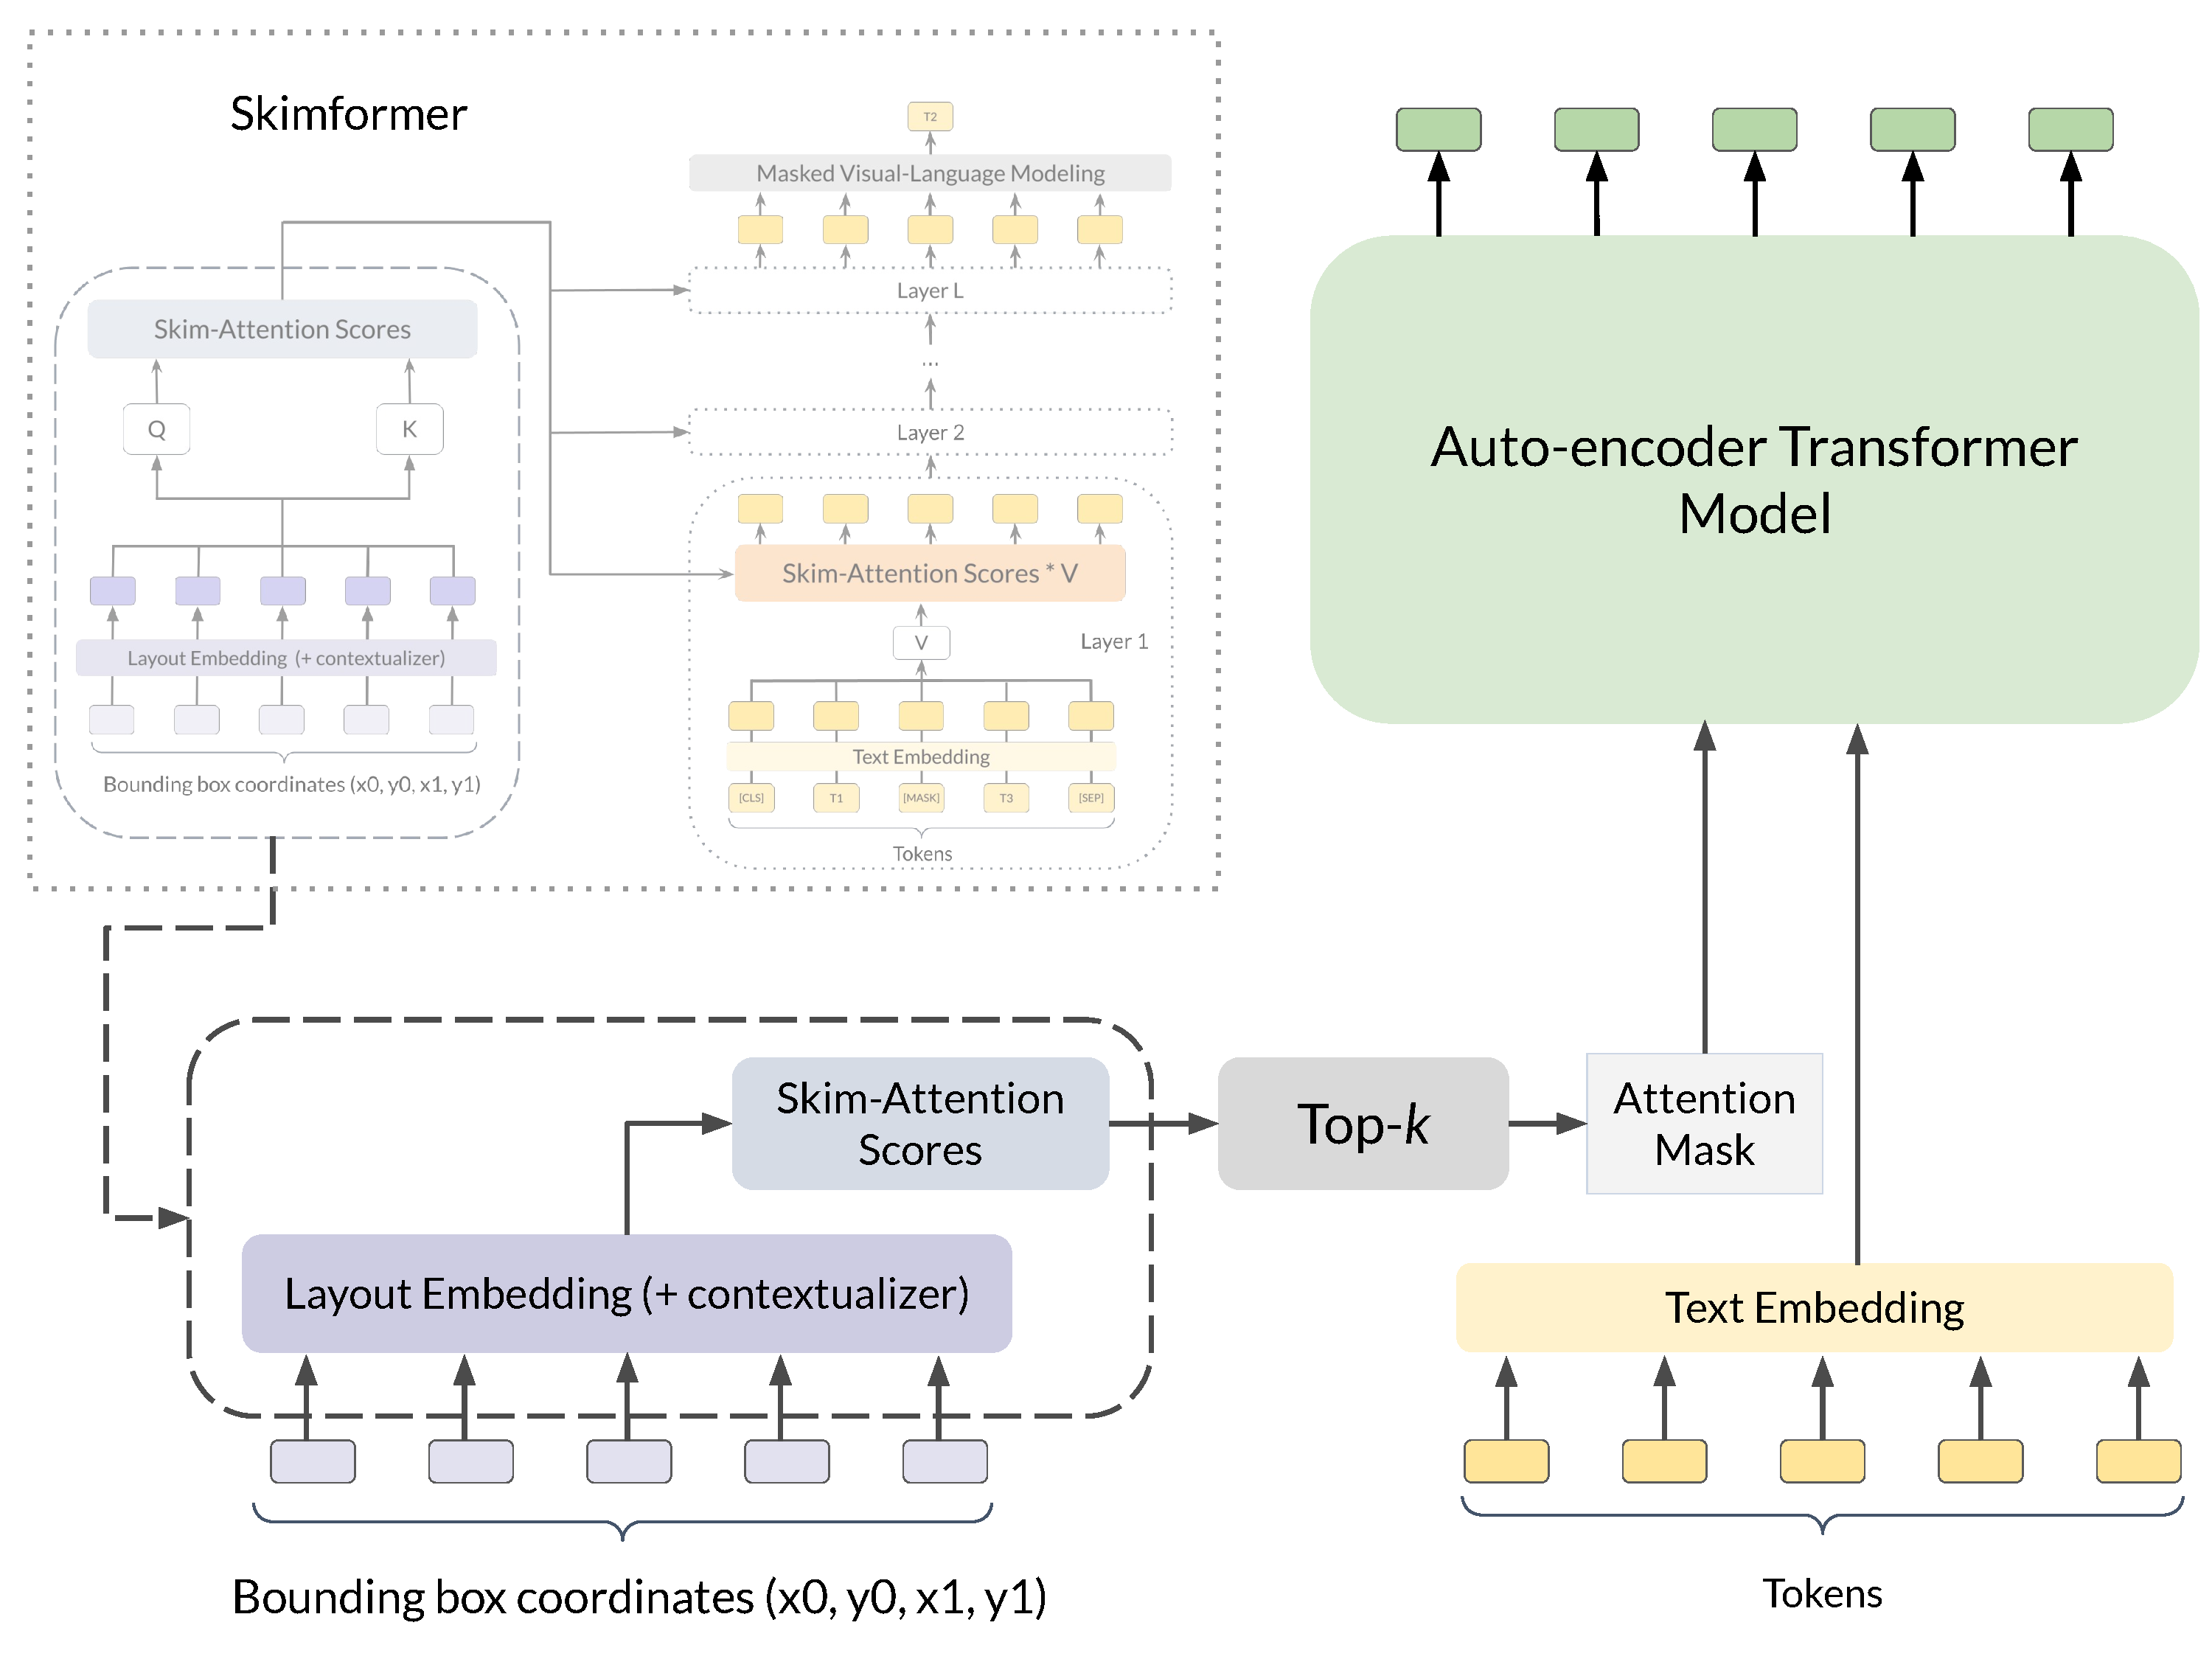
\includegraphics[width=0.7\textwidth]{images/chapter3/skimmingmask-architecture.pdf}
    \caption{Skimming Mask model architecture. The layout embeddings, Key and Query projections are initialized from an already pre-trained Skimformer model. By filtering the $k$ most attended tokens for each token, the Skim-Attention scores are then converted to an attention mask and given as input to a text-based Transformer model.}
    \label{fig:skimmingmask-architecture}
\end{figure}

One drawback of Skimformer is that it does not use attention based on semantics. However, for each token in a sequence, Skim-Attention provides a ranking of every other token in accordance with their layout-based similarity. Drawing from this observation, \emph{Skimming Mask} answers the second question: \textit{Can layout help reduce the complexity of self-attention?} by using Skim-Attention as a \textit{mask} to restrict the computation of self-attention to a smaller number of elements for each token. In this setting, Skim-Attention is viewed as an independent, complementary module that can be plugged into any language model. Given a sequence of layout embeddings, the corresponding skim-attention matrix is converted to an attention mask: based on the similarity scores provided in the attention matrix, each token only attends to at most $k$ tokens. The mask is given as input to a text-based Transformer language model with vanilla self-attention, and is used to restrict self-attention for each element in the input text sequence. This can be viewed as \emph{sparsifying} the standard self-attention matrix. In contrast to the sparse pattern methods discussed in Section~\ref{subsubsection:related-long-range-modeling-sparse}, this sparsity is determined by the document's layout.

It is worth nothing that Skimming Mask introduces a new way to cluster tokens: tokens within the same group have a high similarity to each other in terms of their respective \emph{layout positions}. This characteristic positions Skimming Mask as a concurrent approach to Reformer \citep{kitaev2020reformer}, which reduces the cost of self-attention by clustering tokens into chunks. As opposed to the latter, the concept of similarity is not derived from text semantics but rather from the document structure. Furthermore, Skimming Mask does not require an understanding of the semantic content; it solely relies on their layout features. Because each token is viewed as a bounding box whose characteristics are only its size and position, the representation space of layout features is much smaller than that of the text, which spans a vocabulary of more than 30k sub-words. As a consequence, computing attention based on layout could require a smaller latent space dimension than for text, corresponding to less computational efforts. This is also the case for humans: as demonstrated in section \ref{section:human-evaluation}, it is much easier to retrieve information from documents when the layout is provided.

Ideally, the Skimming Mask pattern should be learned in an end-to-end fashion alongside the Transformer model. However, achieving this end-to-end training in practice is challenging due to the non-differentiable nature of generating an attention mask from an attention matrix. Consequently, to train this model, the weights for Skim-Attention must have already undergone training. In this context, we naturally use the pre-trained Skimformer weights. The overall architecture of the model is illustrated in Figure~\ref{fig:skimmingmask-architecture}.

The computational complexity is reduced to $\mathcal{O}(L'd'n^2 + Ldk^2 + Ldn^2)$, where the first term represents the time required to compute the skim-attention scores, the second term corresponds to the time needed to calculate the sparse attention matrix, and the third term pertains to the time required to compute the residual value for each token in the input. Meanwhile, the memory complexity for Skimming Mask is reduced to $\mathcal{O}((d’n + n^2) + Ldk + Lk^2)$, encompassing the memory requirements for Skim-Attention and those for the sparsified attention mechanism.

\section{Experiments and Results}

We first present the data used to pre-train and evaluate our models, and provide details on the experimental settings. Then, we discuss the results obtained on language modeling and document layout analysis, before exploring the attention maps obtained by Skimformer.

\subsection{Data}

\subsubsection{Pre-training Data}

To pre-train our models on a wide variety of document formats, we select three datasets with various non-trivial document layouts: DocBank \citep{li2020docbank}, RVL-CDIP \citep{harley2015evaluation} and PubLayNet \citep{zhong2019publaynet}. We combine them by randomly selecting 25k documents from each dataset, for a total of 75K documents. We discard the provided labels and consider these data as unannotated. The resulting dataset is referred to as \textit{MIX}. As a first evaluation metric, we can compare the perplexity for the different language models on MIX. 

\paragraph{DocBank}

DocBank is a large-scale dataset that contains 500K English document pages from papers extracted from arXiv.com. These articles span a variety of disciplines (\textit{e.g.}, Physics, Mathematics, and Computer Science), which is beneficial to train more robust models. Pages are split into a training set, validation set and test set with a ratio of 8:1:1. As the authors already extracted the text and bounding boxes using PDFPlumber,\footnote{https://github.com/jsvine/pdfplumber} there is no need for an \ac{OCR} system or a PDF parser. To build our subset, we extract 25k document pages: 20k from the full training set, 2,500 from the validation set and 2,500 from the test set. 

\paragraph{RVL-CDIP}

RVL-CDIP is a large collection of 400k scanned document images from various categories (\textit{e.g.}, letter, form, advertisement, invoice). The wide range of layouts, as well as the low image quality, allows to train more robust models. We select 25k documents from the RVL-CDIP dataset available on Kaggle,\footnote{https://www.kaggle.com/nbhativp/first-half-training} which amounts to half of the training images from the full dataset (160k images). The text and word bounding boxes are extracted using Tesseract \citep{kay2007tesseract}. We split the data into 80\% for training, 10\% for validation and 10\% for test.

\paragraph{PubLayNet}

PubLayNet comprises over 360k document images from PubMed Central\textsuperscript{\texttrademark} Open Access. The medical publications contained in the collection have similar layouts, but the text density coupled with the small image size add to the robustness of the trained models. We arbitrarily extract the first training split among the 7 available on IBM Data Asset eXchange\footnote{https://developer.ibm.com/exchanges/data/all/publaynet/} and use the first 20k images as our training set. For the validation and test sets, we keep the first 2,500 images in each split. Because Tesseract's accuracy is too low without any pre-processing, we apply a few image processing operations (\textit{i.e.}, rescaling, converting to grayscale, applying dilation and erosion) on each image in order to improve text extraction.

\subsubsection{Dataset for Document Layout Analysis}

In addition to perplexity, we evaluate our approach on a downstream task, document layout analysis, which consists in associating each token with its corresponding category. We use a subset of the full DocBank dataset, where the categories are: abstract, author, caption, date, equation, footer, list, paragraph, reference, section, table, title and figure.\footnote{We actually discard the \textit{Figure} label, as 1) our models do not take image features into account, and 2) the text associated with such elements is always the same, making the task trivial.}

The subset is created by selecting 10k document pages (distinct from the ones used for pre-training): 8,000 from the full training set, 1,000 from the validation set and 1,000 from the test set. We refer to this dataset as \textit{DocBank-LA}. Each document page is organized as a list of words with bounding boxes, colors, fonts and labels. We use the precision, recall and F1 score defined by \citet{li2020docbank}.

\subsection{Experimental Settings}

For reproducibility purposes, the code and data pre-processing scripts are made publicly available.\footnote{https://github.com/recitalAI/skim-attention}

\subsubsection{Baselines}

We compare our models with three baselines: i) the text-only \ac{BERT} \citep{devlin2018bert}, ii) the multi-modal LayoutLM \citep{xu2020layoutlm}, and iii) the text-only Longformer \citep{beltagy2020longformer} for long documents. Note that the LayoutLM architecture is based on \ac{BERT}, with additional layout components. For fair comparison, all our models designed for short sequences are based on \ac{BERT} as well, as detailed below. All the models are trained from scratch.

\subsubsection{Pre-training}

For \ac{BERT}, LayoutLM and Longformer, we use their base architecture. Following the \ac{BERT} base model, Skimformer consists of a 12-layer Transformer encoder with 12 attention heads and a hidden size set to 768 for both text and layout embeddings, amounting to 99M parameters. We further add a 2-layer Transformer encoder to contextualize the layout embeddings, which increases the number of parameters to 113M. To test Skim-Attention on longer documents, we build LongSkimformer, a combination of Skim-Attention and Longformer. Every model is trained from scratch on the MIX dataset for 10k steps. We set the maximum sequence length to $n = 512$ for every model except for Longformer and LongSkimformer, for which $n = 2,048$. While \ac{BERT} and Longformer are pre-trained with \ac{MLM}, Skimformer, LongSkimformer and LayoutLM are pre-trained using \ac{MVLM}, an extension of \ac{MLM} that incorporates layout information into the pre-training task. 

\subsubsection{Document Layout Analysis}

As DocBank contains fine-grained token-level annotations, we consider the document layout analysis task as a sequence labeling task. Each model pre-trained on MIX is fine-tuned on this downstream task for 10 epochs. For the Skimming Mask models, we selected the hyperparameter $k$ on the validation set, i.e. the number of tokens that can be attended to. We tested $k \in \{512, 384, 256, 128\}$.

\subsection{Language Modeling Evaluation}

\subsubsection{Perplexity}

\begin{table}
\centering \small
\begin{tabular}{lr}
    \hline
    \textbf{Model} & \textbf{Test Perplexity}\\
    \hline
    \ac{BERT} \citep{devlin2018bert} &  357.11 \\
    LayoutLM \citep{xu2020layoutlm}    & 45.86 \\
    Skimformer                         & 33.77 \\
    \midrule
    Longformer \citep{beltagy2020longformer} & 333.28 \\
    LongSkimformer                     & \textbf{32.02} \\
    \hline
\end{tabular}
\caption{Test perplexity on the MIX dataset after 10k optimization steps. Each model was trained from scratch. Bold denotes the best score.}
\label{tab:ppl-mix}
\end{table}

In Table~\ref{tab:ppl-mix}, we report the perplexity on the MIX dataset. We observe that Skimformer and LongSkimformer outperform both \ac{BERT} and Longformer by a huge margin, while improving perplexity by more than 10 points over LayoutLM. In addition, Figure~\ref{fig:pretraining-learning-curves} demonstrates that Skimformer converges much faster than \ac{BERT}, and slightly more than LayoutLM, indicating its efficiency in learning from the training data. However, it is worth acknowledging certain limitations. Firstly, the models are pre-trained on a relatively small dataset, which may impact their generalizability to larger datasets. Additionally, achieving better perplexity does not always guarantee improved performance in downstream tasks.

\begin{figure}
    \centering \small
    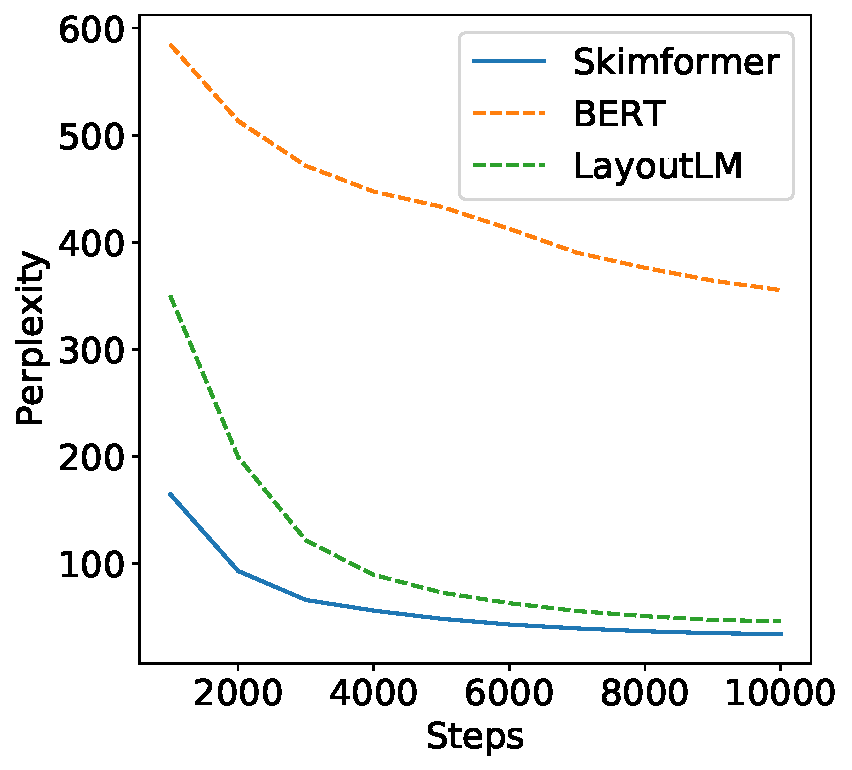
\includegraphics[width=.4\textwidth]{images/chapter3/learning_curves-mix-steps10k-clean2.pdf}
    \caption{Model perplexity on the MIX validation set with respect to the number of optimization steps. All models are trained from scratch.}
    \label{fig:pretraining-learning-curves}
\end{figure}

\subsubsection{Ablation Study}

We further conduct an ablation study about the influence of the Skim-Attention inputs on Skimformer's performance. The results are listed in Table~\ref{tab:ablation-study}. To estimate the impact of the input type, we consider a Skimformer model i) wherein layout representations are not contextualized (\textit{Non-contextualized Layout}), ii) Skim-Attention is based on sequential positions (\textit{1D position}), iii) the bounding boxes are all set to the same fixed value, preventing the model to gather any information about the true location (\textit{Uniform layout}), and iv) they are replaced by their centers (\textit{Degraded layout}). We also provide the perplexity obtained by the full Skimformer model.

\begin{table}[t]
\centering \small
\begin{tabular}{lrr}
    \hline
    \textbf{Skim-Attention Input} & &\textbf{Test Perplexity}\\
    \hline
    Non-contextualized Layout  &                            & 36.41 \\
    1D position    &                     & 54.39 \\ 
    Uniform layout   &                   & 421.97 \\
    Degraded layout    &                 & 103.39 \\
    \hline 
    Full Model  &             & \textbf{33.77} \\
    \hline
\end{tabular}
\caption{Ablation study on the MIX dataset, where perplexity on the test set is reported. All models were trained from scratch. Bold denotes the best score.}
\label{tab:ablation-study}
\end{table}

We find that computing Skim-Attention directly on the layout embeddings (\textit{Non-contextualized Layout}) results in higher perplexity. Additionally, substituting spatial positions with sequential positions (\textit{1D position}) leads to an increase in perplexity, indicating that layout information is crucial for the language model. We also observe that assigning the same bounding box to every token (\textit{Uniform Layout}) leads to a severe drop in performance. Coupled with the perplexity obtained with a degraded layout, this shows that the model's performance is greatly impacted by the layout input quality. 

\subsubsection{Training Speed and Memory Usage}
\label{subsubsection:training-speed-memory-usage}

Using Hugging Face's Transformers benchmarking tools \citep{wolf2019huggingface}, we benchmark Skimformer and LayoutLM on both speed and required memory for pre-training. We consider the base variant of LayoutLM, and use the implementation from the Transformers library. In addition to Skimformer, we evaluate a variant in which the small Transformer contextualizing layout embeddings is removed (\textit{Skimformer-no-context}). The batch size is fixed to 8, and memory and time performance is evaluated for the following sequence lengths: 8, 32, 128 and 512. All experiments were conducted on one Tesla T4 with 15GB of RAM.

% We use Python 3.7.10, PyTorch 1.8.1+cu101 \citep{paszke2019pytorch}, and Transformers 4.6.0.dev0.

Figures~\ref{fig:benchmark-train-time} and \ref{fig:benchmark-train-memory} report the time and peak memory consumption, respectively, with respect to the sequence length. Results show that Skimformer is more time and memory efficient than LayoutLM. 

\begin{figure}[!htbp]
\centering
\small
  \begin{subfigure}[b]{0.49\textwidth}
    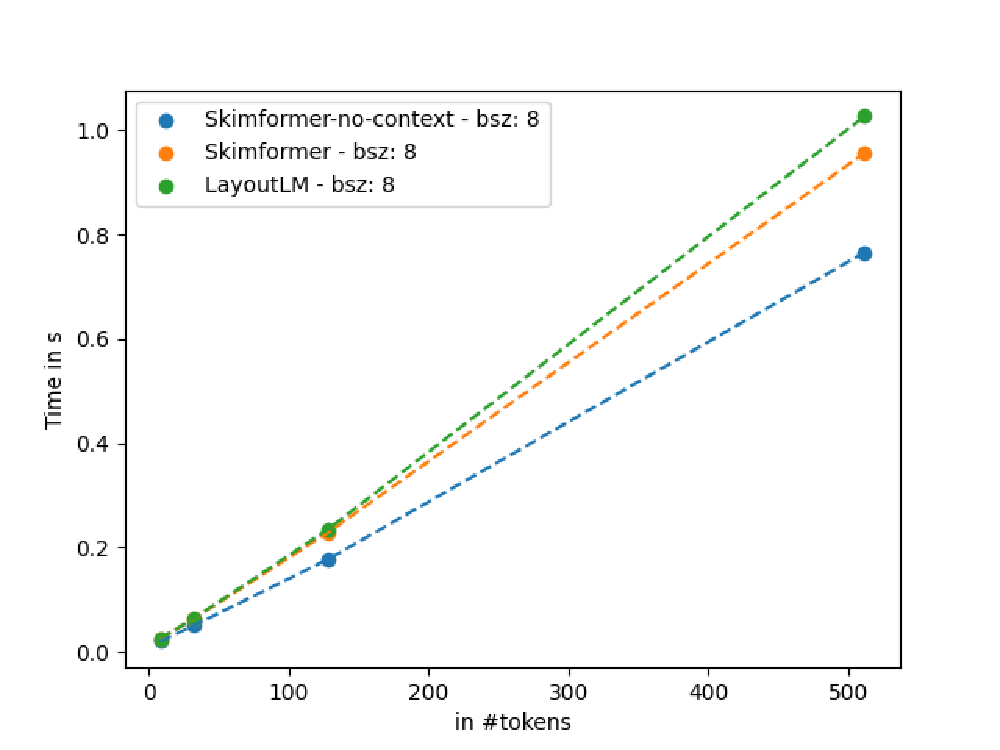
\includegraphics[width=\textwidth]{images/chapter3/train_time_plot.pdf}
    \caption{Time usage for pre-training.}
    \label{fig:benchmark-train-time}
  \end{subfigure}
  \begin{subfigure}[b]{0.49\textwidth}
    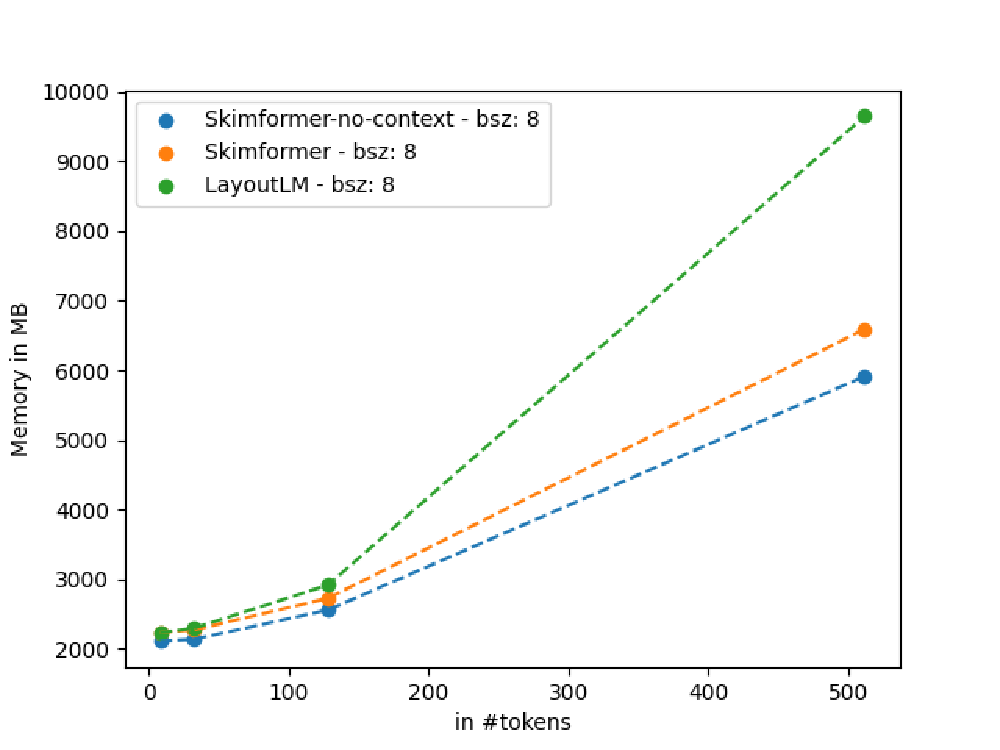
\includegraphics[width=\textwidth]{images/chapter3/train_required_memory_plot.pdf}
    \caption{Memory usage for pre-training.}
    \label{fig:benchmark-train-memory}
  \end{subfigure}
  \caption{Comparison of time and memory usage for LayoutLM (green), Skimformer with layout contextualizer (orange) and without (blue). Results are plotted against sequence length.}
  \label{fig:benchmark}
\end{figure}

\subsection{Document Layout Analysis Evaluation}

\begin{table}
\centering
\small
\begin{adjustbox}{max width=\textwidth}
\begin{threeparttable}
\begin{tabular}{lcccccccc}
    \toprule
     & \textbf{Skimming} & \textbf{Seq.} & \multicolumn{2}{c}{\textbf{Nb Attentions}} & \textbf{Total} & & & \\
    \textbf{Model} & \textbf{Mask} & \textbf{Len} & \textbf{Original}\tnote{*} & \textbf{Skim-Attn} & \textbf{Compute} & \textbf{Rec.} & \textbf{Prec.} & \textbf{F1} \\
    \midrule
    BERT \citep{devlin2018bert}  & \xmark                         & 512 & 12              & 0 & 100.00\% & 67.21 & 59.28 & 60.98 \\ 
    LayoutLM \citep{xu2020layoutlm}        & \xmark                         & 512 & 12              & 0 & 100.00\% & 81.60 & 77.96 & \textbf{79.28} \\
    \midrule 
    Skimformer          & \xmark                         & 512 & 0 & 3\tnote{**} & 25.00\% & 78.80 & 74.35 & 75.86 \\
    BERT+SkimEmbeddings & \xmark                         & 512 & 12              & 0 & 100.00\% & \textbf{82.42} & 77.06 & \textbf{79.16} \\
    
    BERT+SkimmingMask                & \cmark  & 128  & 12  & 3\tnote{**} & 31.25\% & 72.32 & 64.39 & 67.36 \\
    LayoutLM+SkimmingMask              & \cmark & 128 & 12 & 3\tnote{**} & 31.25\% & 81.15 & \textbf{78.30} & \textbf{79.26} \\ 
    \midrule 
    Longformer \citep{beltagy2020longformer} & \xmark & 2,048 & 12 & 0 & 100\% & 74.88 & 69.29 & 71.17 \\
    LongSkimformer & \xmark & 2,048 & 0 & 3\tnote{**} & 25\% & 81.22 & 73.45 & 76.61 \\
\bottomrule
\end{tabular}
\begin{tablenotes}
  \item[*] Standard self-attention for Skimformer, BERT-based and LayoutLM-based models. Longformer self-attention for Longformer and LongSkimformer.
  \item[**] Attention is computed twice (by a 2-layer Transformer) during layout contextualization, then once by Skim-Attention.
\end{tablenotes}
\end{threeparttable}
\end{adjustbox}
\caption{Model performance (in \%) on the DocBank-LA dataset. \textit{Seq. Len} indicates the number of tokens attended with either standard attention (for Skimformer, BERT-based and LayoutLM-based models), or Longformer attention (for Longformer and LongSkimformer). \textit{Nb Attention} represents the number of times attention (original and Skim-Attention) is computed and stored. \textit{Total Compute} specifies the ratio of the final computational cost (\# operations needed to compute attention) w.r.t. BERT/LayoutLM or Longformer. Each model was pre-trained from scratch on the MIX dataset, then fine-tuned on DocBank-LA. }
\label{table:results-docbank}
%\vspace{-0.5cm}
\end{table}

Table~\ref{table:results-docbank} reports the performance on DocBank-LA, the sequence length processed, the number of times attention is computed and the ratio of the total calculation unit ($n^2 \times \textrm{Nb Skim-Attn} + \textrm{Seq. Len}^2 \times \textrm{Nb Standard Attn}$, where $n$ is the length of the initial sequence on which Skim-Attention is applied; and \textit{Seq. Len} is the length obtained after applying Skimming Mask) to that of \ac{BERT}/LayoutLM and Longformer. All models were pre-trained from scratch on MIX. 

Skimformer is substantially superior to \ac{BERT}, improving the F1 score by 15\% while reducing the number of attentions computed by four. We experimented with plugging the layout embeddings learnt by Skimformer in a \ac{BERT} model. The resulting model, BERT+SkimEmbeddings, resembles LayoutLM in terms of architecture.\footnote{In BERT+SkimEmbeddings, the layout embeddings are first projected into the same dimensional space as the text embeddings. In this way, we can plug the layout embeddings from any Skimformer model, in particular smaller ones.} Results show that BERT+SkimEmbeddings performs on par with LayoutLM despite simply combining separately pre-trained modalities, as opposed to the latter which requires an extensive joint training.

For the Skimming Mask models, the models attend only to the top-$k$ 128 tokens. Compared to LayoutLM, this reduction to the quadratic factor allows to obtain the same downstream results with only 31.25\% of the computational burden.
Compared to \ac{BERT}, it even obtains an absolute improvement of more than 6\% in term of F1 score.

LongSkimformer benefits from both Skim-Attention and Longformer's gain in efficiency. It outperforms Longformer by 5\% while requiring four times less attention operations, and the use of Longformer's linear attention allows LongSkimformer to process sequences four times larger than Skimformer can.

Overall, the competitive results achieved by Skimformer show that it is possible to learn attention solely from layout information. Additionally, the efficiency gains and effectiveness demonstrated by the Skimming Mask approach emphasize the potential of leveraging layout information to reduce the complexity of self-attention.

\subsection{Attention Visualization}
\label{subsection:attention-visualization}

\begin{figure}
    \centering \small
    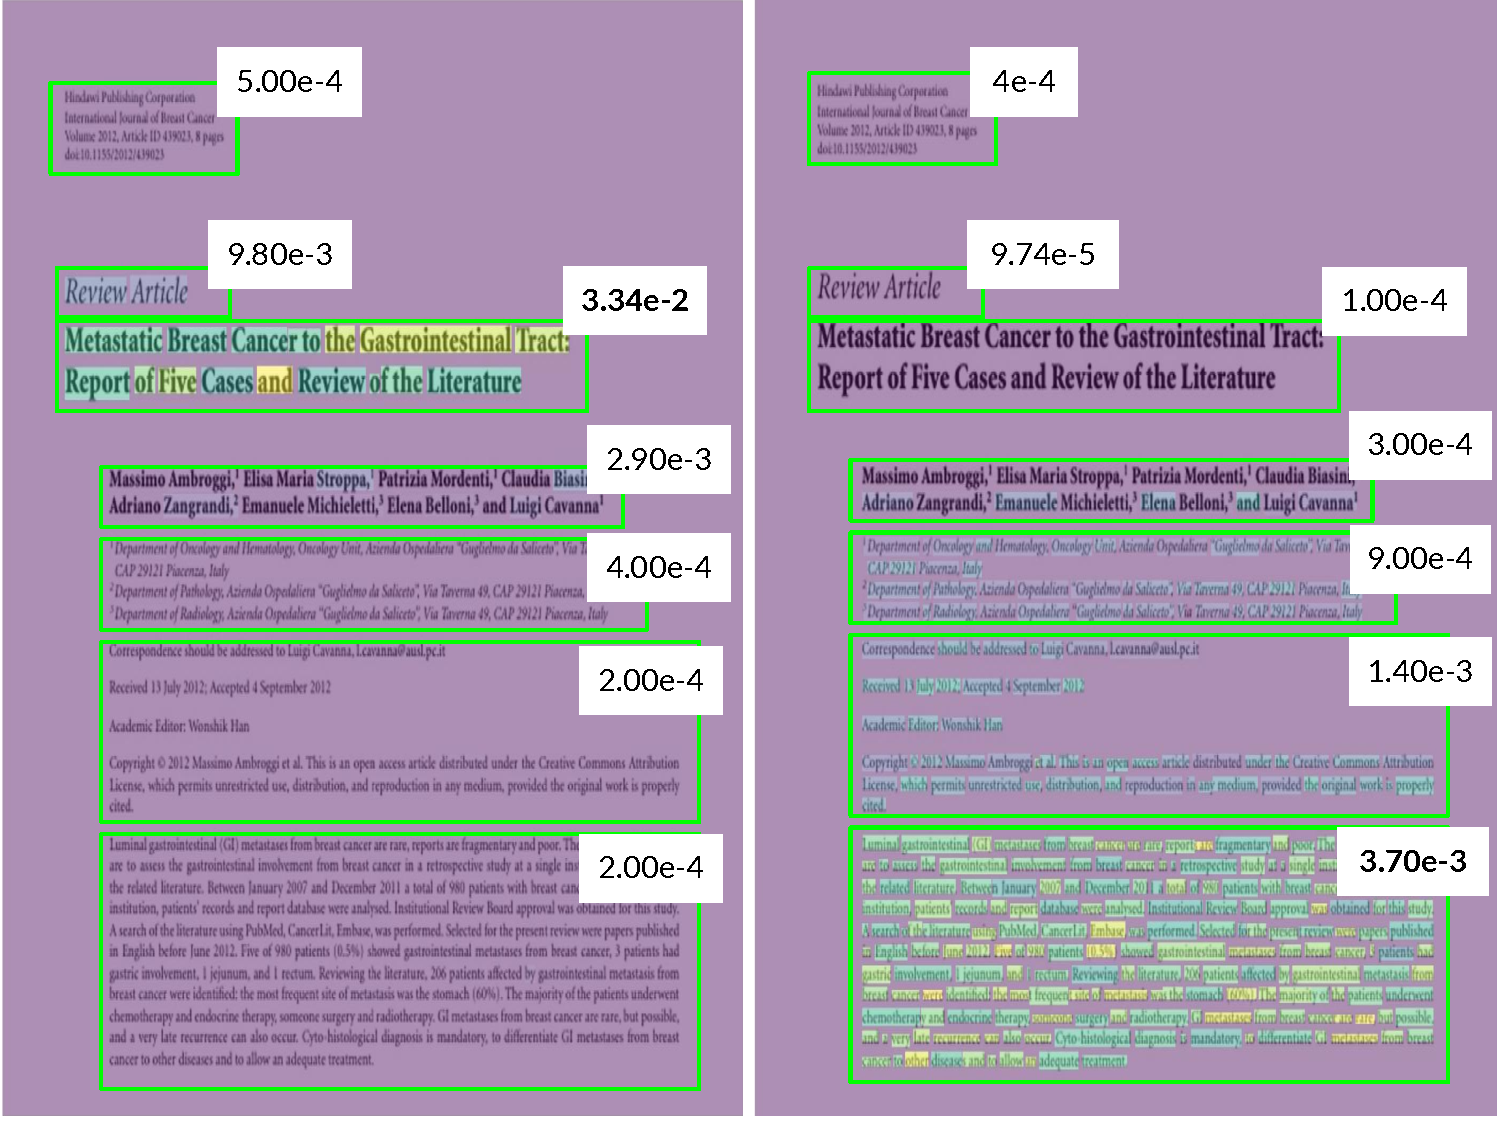
\includegraphics[width=.49\textwidth]{images/chapter3/attention-maps_with-average.pdf}
    \caption{Skim-attention maps corresponding to the title (left) and the abstract (right), along with average attention score (in white) per text block (in green). We consider the skim-attention matrix averaged over all the attention heads. Given a semantic unit (title or abstract), we plot the average attention score for each token.
    }
    \label{fig:attention-vis}
    % \vspace{-0.5cm} 
\end{figure}

Figure~\ref{fig:attention-vis} shows the attention maps produced by Skimformer on a randomly sampled document. Given a semantic unit (either title or abstract in our example), we select the corresponding tokens and compute their average attention over the whole document. We observe, both qualitatively and quantitatively, that tokens attend mainly to other elements in the same semantic unit, thus creating clusters of tokens that are relevant to each other. This shows that the model has grasped the concept of semantic unit with only self-supervision, enabling the emergence of a document structure representation. We argue that these structure-aware clusters could pave the way for long text encoding and unsupervised document segmentation.

\section{Conclusion}

We have presented Skim-Attention, a novel structure-aware attention mechanism. Distinct from prior works in layout-aware pre-training, Skim-Attention builds on cognitive science: rather than considering every single token in the document to compute attention, our approach exploits 2D positions. We conduct extensive experiments to show the effectiveness of Skim-Attention, both as an end-to-end model (Skimformer) and as a mask for any language model (Skim-Attention). 

Potential extensions of this work include full-scale pre-training, integrating image features into Skim-Attention to leverage information across all modalities, as well as exploring tasks that require capturing longer-range dependencies.

Most pre-trained language models depend on serialized text obtained through \ac{OCR} or PDF parsing. Yet, accurately detecting the \textit{reading order} of visually-rich documents poses a significant challenge. With the aim of advancing models that capture document structure more intuitively, the next chapter will focus on addressing reading order issues by leveraging document layout and entirely discarding sequential position information.


